\documentclass[../../main.tex]{subfiles}
\begin{document}

\begin{flushright}
\footnotesize\textit{【自動文字起こし・要確認】}
\end{flushright}

\noindent
[\textbf{解}] (1) $a$ 以外の2辺の長さを $x, y$ とする。この時、$x + y = m$ に注意する。

\noindent
$S = \dfrac{1}{2}(x+y+a) = \dfrac{1}{2}(m+a)$ としてヘロンの公式から、面積 $T$ として
\begin{align}
T &= \sqrt{S(S-x)(S-y)(S-a)} \\
&\le \sqrt{S(S-a)} \cdot \dfrac{(S-x)+(S-y)}{2} \quad (\because S-x, S-y > 0 \text{ から AM-GM}) \\
&= \sqrt{S(S-a)} \cdot \dfrac{2S-m}{2}
\end{align}
等号成立は $S-x = S-y \therefore x=y=\dfrac{m}{2}$ の時。つまり、この時三角形は2等辺三角形である。

\bigskip
\noindent
[\textbf{解2}] $\angle BAC + \angle BDC = \theta$ とする。

\begin{center}
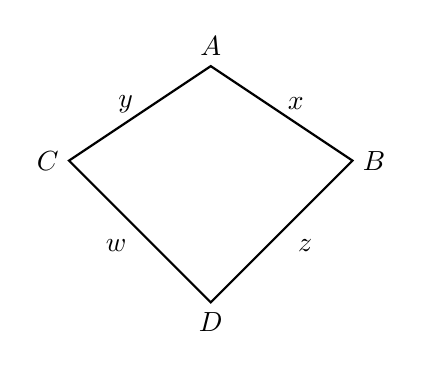
\begin{tikzpicture}[scale=1.2]
    \coordinate (A) at (0, 1.5);
    \coordinate (B) at (1.5, 0.5);
    \coordinate (C) at (-1.5, 0.5);
    \coordinate (D) at (0, -1.0);
    \draw[thick] (A) node[above]{$A$} -- (B) node[right]{$B$} -- (D) node[below]{$D$} -- (C) node[left]{$C$} -- cycle;
    \node at (-0.9, 1.1) {$y$};
    \node at (0.9, 1.1) {$x$};
    \node at (-1.0, -0.4) {$w$};
    \node at (1.0, -0.4) {$z$};
\end{tikzpicture}
\end{center}

\noindent
ブレードシュナイダーの公式から、$S = \dfrac{1}{2}(x+y+z+w) = \dfrac{1}{2}m$ として
\begin{align}
T &= \sqrt{(S-x)(S-y)(S-z)(S-w) - xyzw \cos^2 \dfrac{\theta}{2}} \\
&\le \sqrt{ \left\{ \dfrac{(S-x)+(S-y)+(S-z)+(S-w)}{4} \right\}^4 } \quad (\because \text{AM-GM 及び } xyzw \cos^2 \dfrac{\theta}{2} \ge 0) \\
&= \dfrac{m^2}{16}
\end{align}
等号成立は $x=y=z=w$ かつ $\theta=\pi$、つまり $\square ABCD$ が正方形の時。

\bigskip
\noindent
(2) 四角形 $ABCD$ とし、4辺の長さを $x, y, z, w$ とする。この時、$m$ を定数 ($>0$) として
\[
x + y + z + w = m \quad \dots \text{①}
\]
となる。$|BC| = a\ (>0)$, $x+y = k\ (k > a)$ と固定すると、$\triangle ABC$, $\triangle BCD$ は $x=y, z=w$ の時 面積最大である。この面積を $S(k)$ とする。右下図から ($E$ は $BC$ の中点)

\begin{center}
\begin{tikzpicture}[scale=1.2]
    \coordinate (A) at (0, 1.8);
    \coordinate (B) at (1.2, 0);
    \coordinate (C) at (-1.2, 0);
    \coordinate (D) at (0, -1.2);
    \coordinate (E) at (0, 0);
    \draw[thick] (A) node[above]{$A$} -- (B) node[right]{$B$} -- (D) node[below]{$D$} -- (C) node[left]{$C$} -- cycle;
    \draw[dashed] (C) -- (B);
    \draw[dashed] (A) -- (D);
    \fill (E) circle (1.5pt) node[above right]{$E$};
    \node at (-0.6, 0.15) {$\dfrac{a}{2}$};
    \node at (0.6, 0.15) {$\dfrac{a}{2}$};
    \node at (-0.9, 1.0) {$\dfrac{k}{2}$};
    \node at (0.9, 1.0) {$\dfrac{k}{2}$};
    \node at (-1.0, -0.7) {$\dfrac{m-k}{2}$};
    \node at (1.0, -0.7) {$\dfrac{m-k}{2}$};
\end{tikzpicture}
\end{center}

\begin{align}
S(k) &= \dfrac{1}{2} a (\overline{AE} + \overline{ED}) \\
&= \dfrac{1}{2} a \left\{ \sqrt{\left(\dfrac{k}{2}\right)^2 - \left(\dfrac{a}{2}\right)^2} + \sqrt{\left(\dfrac{m-k}{2}\right)^2 - \left(\dfrac{a}{2}\right)^2} \right\} \\
&\le \dfrac{1}{2} a \sqrt{(1+1) \left\{ \left(\dfrac{k}{2}\right)^2 - \left(\dfrac{a}{2}\right)^2 + \left(\dfrac{m-k}{2}\right)^2 - \left(\dfrac{a}{2}\right)^2 \right\}} \quad (\because \text{コーシー・シュワルツ, 等号成立は } k = \dfrac{1}{2}m) \\
&= \dfrac{1}{2} a \sqrt{k^2 - mk + \dfrac{1}{2}m^2 - a^2} \\
&= \dfrac{1}{2} a \sqrt{\left(k - \dfrac{1}{2}m\right)^2 + \dfrac{1}{4}m^2 - a^2} \\
&\le \dfrac{1}{2} a \sqrt{\dfrac{1}{4}m^2 - a^2} \quad (\text{等号成立は } k = \dfrac{1}{2}m)
\end{align}
だから、$a$ を固定した時、$k = \dfrac{1}{2}m$ で $S(k)$ は $\max \dfrac{1}{2} a \sqrt{\dfrac{1}{4}m^2 - a^2}$ をとる。($\dfrac{1}{2}m > a$ は満たしている)

\noindent
次に $a$ を動かす。($0 < a < \dfrac{1}{2}m$)
\begin{align}
S(k) &= \dfrac{1}{2} \sqrt{ -a^4 + \dfrac{1}{4}m^2 a^2 } \\
&= \dfrac{1}{2} \sqrt{ -\left(a^2 - \dfrac{1}{8}m^2\right)^2 + \dfrac{1}{64}m^4 } \\
&\le \dfrac{1}{16} m^2 \quad (\text{等号成立は } a = \dfrac{\sqrt{2}}{4}m \text{ のとき})
\end{align}
したがって $S(k)$ は $a = \dfrac{\sqrt{2}}{4}m \ (0 < \dfrac{\sqrt{2}}{4}m < \dfrac{1}{2}m)$ で $\max$。

\noindent
この時、$x = y = z = w = \dfrac{1}{4}m, a = \dfrac{\sqrt{2}}{4}m$ で、たしかに $\square ABCD$ は正方形である。

\noindent
以上から示された。

\newpage

\end{document}
